\documentclass[10pt]{beamer}

\usepackage[utf8]{inputenc}
\usepackage[T1]{fontenc}
\usepackage[french]{babel}
\usepackage[ddmmyyyy]{datetime}
\usepackage{listings,lstautogobble,graphicx,tikz}
\usepackage{lmodern}
\usetikzlibrary{arrows,automata}
\usetikzlibrary{positioning}

\usetheme{Warsaw}
\useinnertheme{rectangles}
\setbeamerfont{headline}{size=\large}
\setbeamerfont{frametitle}{size=\normalsize}

%Plan/Sommaire automatique avant chaque section
\AtBeginSection[]{
  \begin{frame}
  \frametitle{Plan}
  \tableofcontents[currentsection]
  \end{frame}
}

\author{Jean-Didier Pailleux - Robin Feron - Romain Robert - Damien Thenot - Maxence Joulin}
\institute{UVSQ}
\date{\today}
\usepackage{../tex/myInfolines}
\usepackage{graphicx}
\usepackage{algorithm}
\usepackage{algorithmic}
\usepackage{subcaption}
\usepackage{longtable,array}
\newenvironment{figure*}%
{\begin{figure}}
{\end{figure}}
\title{Test de Primalité}

\begin{document}
	\begin{frame}
		\titlepage
	\end{frame}
	
	\section*{Introduction}
        \begin{frame}
                    
        \end{frame}
	
	\begin{frame}
		\tableofcontents
	\end{frame}
	
	\section{Optimisation}
	\begin{frame}
	
	\end{frame}
	
	\section{Parallélisation}
	\begin{frame}
	
	\end{frame}
	
	\section{Résultats}
	\begin{frame}
	
	\begin{figure}[!ht]	
		\begin{center}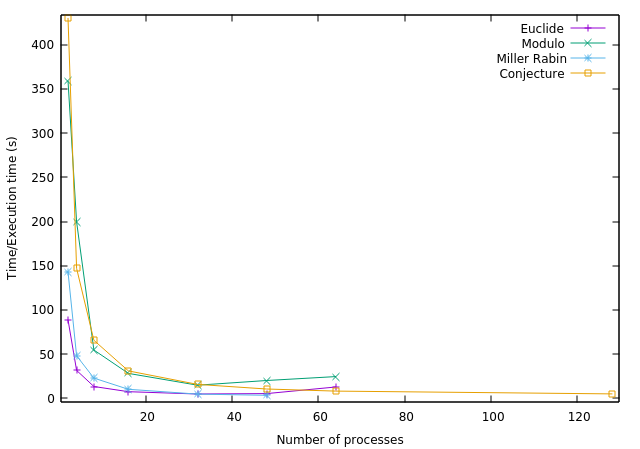
\includegraphics[scale=0.5]{All_1M.png}\end{center}
		\caption{Évolution du temps de calcul pour Conjecture, Miller-Rabin, Euclide et Modulo; Plage [1, 1 000 000]}
		\label{fg:fig1}
	\end{figure}
	\end{frame}

	\begin{frame}
	\begin{figure}[!ht]	
		\begin{center}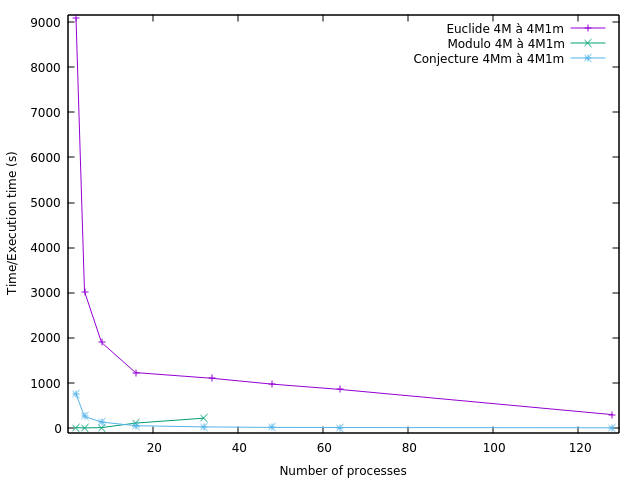
\includegraphics[scale=0.5]{All_4M.png}\end{center}
		\caption{Évolution du temps de calcul pour Conjecture, Euclide et Modulo; Plage [4M, 4M1m]}
		\label{fg:fig2}
	\end{figure}	
	\end{frame}
	
	\begin{frame}
	\begin{figure}[!ht]	
		\begin{center}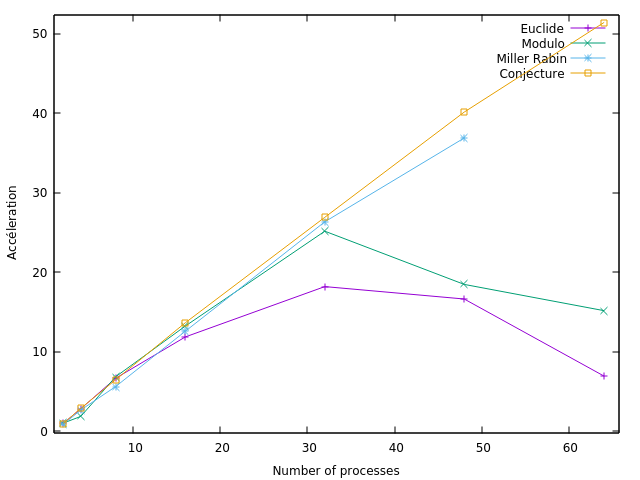
\includegraphics[scale=0.55]{Acc_All_1M_v2.png}\end{center}
		\caption{Évolution de l’accélération en fonction du nombre de processus sur Plage [1, 1 000 000].}
		\label{fg:fig4}
	\end{figure}	
	\end{frame}
		
	\begin{frame}
	\begin{figure}[!ht]	
		\begin{center}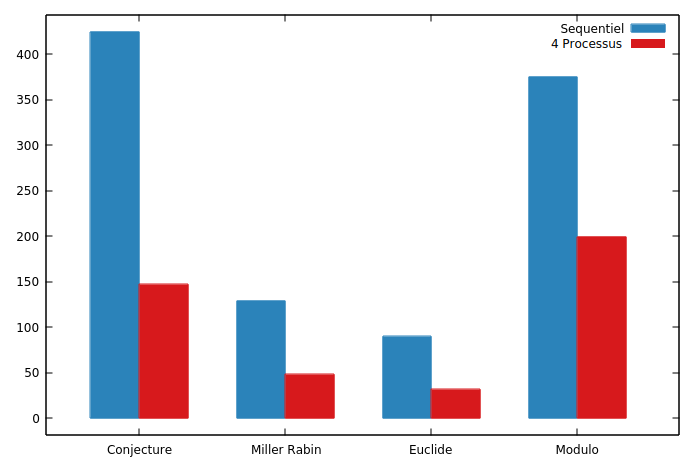
\includegraphics[scale=0.4]{Bar1.png}\end{center}
		\caption{Comparaison Conjecture, Miller-Rabin, Euclide et Modulo avec le séquentiel}
		\label{fg:fig3}
	\end{figure}	
	\end{frame}
		
	\begin{frame}
	\begin{figure}[!ht]	
		\begin{center}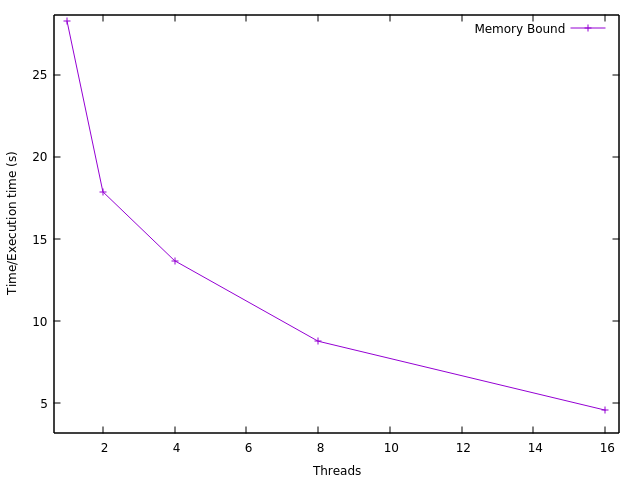
\includegraphics[scale=0.5]{Memory.png}\end{center}
		\caption{Évolution du temps de calcul pour Memory Bound en fonction du nombre de threads.}
		\label{fg:fig4}
	\end{figure}	
	\end{frame}
	
	\begin{frame}
	\begin{figure}[!ht]	
		\begin{center}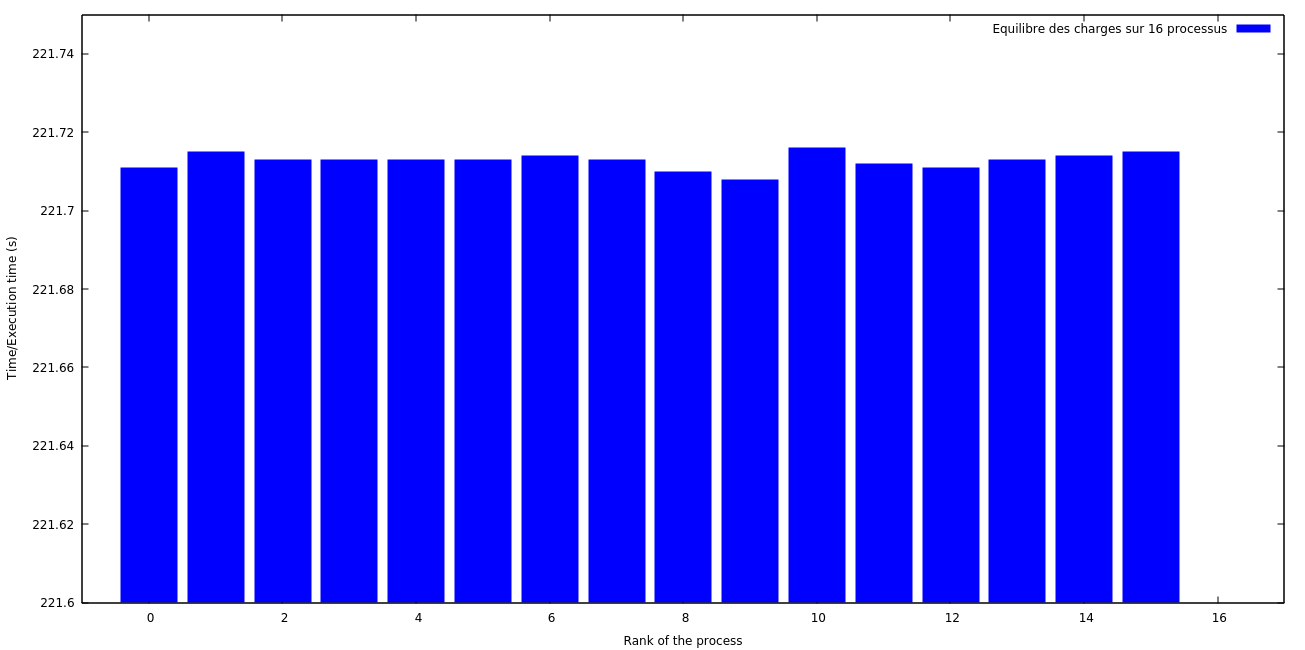
\includegraphics[scale=0.35]{equilibre8.png}\end{center}
		\caption{Exemple d'équilibre des charges obtenu avec 16 processus MPI.}
		\label{fg:fig4}
	\end{figure}	
	\end{frame}
	
	\begin{frame}
	\begin{figure}[!ht]	
		\begin{center}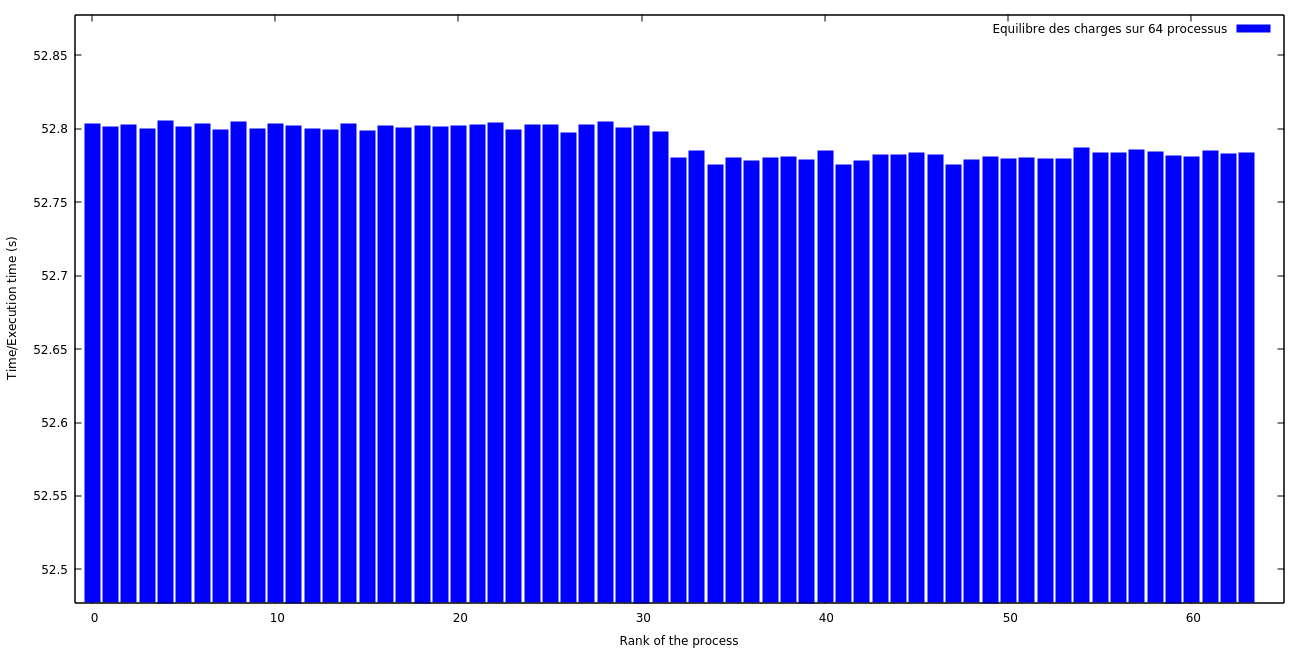
\includegraphics[scale=0.35]{equilibre64.png}\end{center}
		\caption{Exemple d'équilibre des charges obtenu avec 64 processus MPI.}
		\label{fg:fig4}
	\end{figure}	
	\end{frame}
	
	\section{Bilan Technique}
	\begin{frame}
	
	\end{frame}
	
	\section{Problèmes Rencontrés}
	\begin{frame}
	
	\end{frame}
	
	\section{Conclusion}
	\begin{frame}
	
	\end{frame}
\end{document}

% Courbes Accélération sur graphes Bar / Calcul de l'accélération
% Préciser à l'oral que les résultats => 10 runs
% Graphe pour l'équilibre des charges
% Graphes de natures différentes.\\
% Accélération ( 5 courbes => 5 accélérations) par rapport au temps séquentiel
% Implem paralléle non-existante (rappel) 
% Parler de l'algorithme de Master-Slave
% Graphe montrant/décrire le Master-Slave( Mettre le graphe après les résultats => transition sur le bilan ?)
% Problèmes avant les Bilan tech/ Ou l'inverse
% Test avec 999995819